% -*- latex -*-
%-----------------------------------------------------------------------
%;  Copyright (C) 2005
%;  Associated Universities, Inc. Washington DC, USA.
%;
%;  This program is free software; you can redistribute it and/or
%;  modify it under the terms of the GNU General Public License as
%;  published by the Free Software Foundation; either version 2 of
%;  the License, or (at your option) any later version.
%;
%;  This program is distributed in the hope that it will be useful,
%;  but WITHOUT ANY WARRANTY; without even the implied warranty of
%;  MERCHANTABILITY or FITNESS FOR A PARTICULAR PURPOSE.  See the
%;  GNU General Public License for more details.
%;
%;  You should have received a copy of the GNU General Public
%;  License along with this program; if not, write to the Free
%;  Software Foundation, Inc., 675 Massachusetts Ave, Cambridge,
%;  MA 02139, USA.
%;
%;  Correspondence concerning AIPS should be addressed as follows:
%;          Internet email: aipsmail@nrao.edu.
%;          Postal address: AIPS Project Office
%;                          National Radio Astronomy Observatory
%;                          520 Edgemont Road
%;                          Charlottesville, VA 22903-2475 USA
%-----------------------------------------------------------------------
%Body of intermediate AIPSletter for 31 December 2005

\documentclass[twoside]{article}
\usepackage{graphics}

\newcommand{\AIPRELEASE}{June 30, 2005}
\newcommand{\AIPVOLUME}{Volume XXV}
\newcommand{\AIPNUMBER}{Number 1}
\newcommand{\RELEASENAME}{{\tt 31DEC05}}
\newcommand{\NEWNAME}{{\tt 31DEC05}}
\newcommand{\OLDNAME}{{\tt 31DEC04}}

%macros and title page format for the \AIPS\ letter.
\input LET98.MAC
%\input psfig

\newcommand{\MYSpace}{-11pt}

\normalstyle

\section{General developments in \AIPS}

\subsection{Current and future releases}

We now have formal \AIPS\ releases on an annual basis.  Beginning near
the end of 2004, we have made available full binary installation
methods for both the frozen and development versions  for MacIntosh
OS/X, Solaris, and Linux.  All architectures can do a full
installation from the source files.  The next release is called
\RELEASENAME\ and remains under active development.  You may fetch
and install a copy of this version at any time using {\it anonymous}
{\tt ftp} for source-only copies and {\tt rsync} for binary copies.
This \Aipsletter\ is intended to advise you of developments to date in
this new release. Having fetched \RELEASENAME, you may update your
installation whenever you want by running the so-called ``Midnight
Job'' (MNJ) which uses transaction files to copy and compile the code
selectively based on the code changes and compilations we have done.
The MNJ will also update sites that have done a binary installation
using {\tt rsync}.  There is a guide to the install script and an
\AIPS\ Manager FAQ page on the \AIPS\ web site.

The MNJ has been changed.  It now serves up \AIPS\ incrementally using
the Unix tool {\tt cvs} running with anonymous ftp.  The binary MNJ
also uses the tool {\tt rsync} as does the binary installation.  Linux
sites will almost certainly have {\tt cvs} installed; other sites may
have installed it along with other GNU tools.  Secondary MNJs will
still be possible using {\tt ssh} or {\tt rcp} or NFS as with previous
releases.  We have found that {\tt cvs} works very well, although it
has one quirk.  If a site modifies a file locally but in an
\AIPS-standard directory, {\tt cvs} will detect the modification and
attempt to reconcile the local version with the NRAO-supplied version.
This usually produces a file that will not compile or run as intended.

\AIPS\ is now copyright \copyright\ 1995 through 2005 by Associated
Universities, Inc., NRAO's parent corporation, but may be made freely
available under the terms of the Free Software Foundation's General
Public License (GPL)\@.  This means that User Agreements are no longer
required, that \AIPS\ may be obtained via anonymous ftp without
contacting NRAO, and that the software may be redistributed (and/or
modified), under certain conditions.  The full text of the GPL can be
found in the \texttt{15JUL95} \Aipsletter, in each copy of \AIPS\
releases, and on the web at {\tt
  http://www.aoc.nrao.edu/aips/COPYING}.
\vfill\eject

\section{Patch Distribution for \OLDNAME}

Important bug fixes and selected improvements in \OLDNAME\ can be
downloaded via the Web beginning at:

\begin{center}
\vskip -10pt
{\tt http://www.aoc.nrao.edu/aips/patch.html}
\vskip -10pt
\end{center}

Alternatively one can use {\it anonymous} \ftp\ to the NRAO server
{\tt ftp.aoc.nrao.edu}.  Documentation about patches to a release is
placed on this site at {\tt pub/software/aips/}{\it release-name} and
the code is placed in suitable subdirectories below this.  As bugs in
\NEWNAME\ are found, they are simply corrected since \NEWNAME\ remains
under development.  Corrections and additions are made with a midnight
job rather than with manual patches.

The patch system has changed because we now have binary installations.
We now actually patch the master version of \OLDNAME, which means that
a MNJ run on \OLDNAME\ after the patch will fetch the corrected code
and/or binaries rather than failing.  Also, installations of \OLDNAME\
after the patch date will contain the corrected code.

The \OLDNAME\ release had a few important patches most of which were
released in April when we changed the patch system.  These were:
\begin{enumerate}
\item\ {\tt OTFUV, OTFIN} to handle both byte orders of 12m OTF
      data {\it 2005-01-06}
\item\ {\tt CXPOLN} procedure, {\tt CXCLN} task need
      modern image names {\it 2005-04-22}
\item\ {\tt TVFLG} and {\tt SPFLG} required improved
      error handling and modern {\tt FLAGVER} default
      {\it 2005-04-22}
\item\ {\tt WIPER} function {\tt FLAG AREA} aborted on
      wrong button push {\it 2005-04-22}
\item\ {\tt FIXBX} could handle complicated cases but not simple
      ones {\it 2005-04-22}
\item\ {\tt POSSM} used wrong units in output text file
      {\it 2005-04-22}
\item\ {\tt CL2HF} aborts under Linux {\it 2005-04-22}
\item\ {\tt TCOPY} used wrong (old) tape LUNs {\it 2005-04-22}
\item\ {\tt BPASS} gets wrong solutions when channel 1 of of the
      first source was flagged {\it 2005-04-22}
\end{enumerate}

\section{Binary installations are easy}

The \AIPS\ binary installation is so easy that it has confused
would-be installers.  All one really needs to do is visit the web page

\begin{center}
\vskip -12pt
{\tt http://www.aoc.nrao.edu/aips/dec05.shtml}
\vskip -12pt
\end{center}

and read the instructions.  From this page, download the file {\tt
install.pl} putting it in the area you intend to use as {\tt
\$AIPS\_ROOT}.  Then type the instruction

\begin{center}
\vskip -12pt
{\tt \Large perl install.pl -n}
\vskip -12pt
\end{center}

You will be asked some of the usual questions (see the guide to the
Install Wizard available from the cited web page), but with the {\tt
  -n} option, the script will skip fetching and unpacking the tar-ball
and the compiler queries and usage.  It does a variety of {\tt rsync}
commands to fetch a complete copy of the \AIPS\ version including
libraries and all executables.  It marks the installation as a binary
one by creating a special 0-byte file in {\tt \$SYSLOCAL}\@. The MNJ
then detects this file and replaces the compile steps with {\tt rsync}
operations on the binary areas.  Your firewall must allow you to use
the {\tt rsync} and {\tt cvs} utilities (ports 873 and 2401,
respectively) which are used for installing and updating the binary
and text files.
\vfill\eject

\section{Recent \AIPS\ and related Memoranda}

The following new \AIPS\ Memorandum is available from the \AIPS\ home
page.

\begin{tabular}{lp{5.8in}}
111 &  {\tt ATMCA}: Phase Referencing using more than one Calibrator\\
   &    Edward Fomalont \&\ Leonid Kogan, (NRAO)\\
   &   January 6, 2005\\
   &   The VLBI astrometric accuracy and image quality of a target
       source can be improved if more than one reference calibrator is
       observed with the target.  The improvement is obtained by
       determining the phase gradient in the sky in the region of the
       sources, mostly caused by an inaccuracy of the troposphere
       model.  Even if the target is sufficiently strong to use
       self-calibration methods to determine the image, its precise
       location can be improved with phase referencing.  This memo
       describes the scheduling strategy for multi-calibrator phase
       referencing, the reduction of the data, and the use of a new
       \AIPS~task {\tt ATMCA}, which combines the phase or multi-band
       delay information from the several calibrators.
\end{tabular}

The following new EVLA Memorandum is available from the NRAO web
pages.

\begin{tabular}{lp{5.8in}}
93  & Optimization of the LWA Antenna Station Configuration Minimizing
      Side Lobes \\
   & Leonid Kogan \&\ Aaron Cohen\\
   & May 4, 2005\\
   & This memo is a duplicate of LWA memo \#21 and is posted here as
      well because of its relevance to the optimization of the EVLA
      phase II arrays.  The algorithm for optimization of an array
      configuration to minimize side lobes, designed by Leonid Kogan,
      has been applied to optimize the configuration of a dipole
      station of the Long Wavelength Array (LWA). The results of
      optimization are given for different areas of optimization on
      the sky including full sky semi-sphere; for different minimum
      spacing between the station antennas.  For an array phased to
      zenith, the optimization is done to minimize sidelobes all the
      way to the horizons by optimizing in a circle defined by the
      radius $|\sin(z)|\leq 1$, where $z$ is the angle from zenith.
      {\em For an array that will potentially be phased to any
      location above the horizon, the optimization radius should be
      twice as large to optimize the beam pattern over the entire
      sky.}  Thus for the whole semisphere optimization with a range
      of array pointings covering the whole semisphere as well,
      optimization at zenith pointing must be done for $|\sin(z)|\leq
      2$ !
\end{tabular}

The following paper has been approved for inclusion in the FITS
Standard by the regional committees.  Submission to {\it A\&A}, {\it
  astroph},  and the IAU FITS Committee will follow.  It is currently
available from Eric Greisen's home page:
{\tt http://www.aoc.nrao.edu/$\sim$egreisen}

\begin{tabular}{lp{5.8in}}
III & Representations of spectral coordinates in FITS \\
   & E. W. Greisen (NRAO), M. R. Calabretta (ATNF),
        F. G. Valdes (NOAO), and S. L. Allen (UCO/Lick)\\
   & 24 May 2005\\
   & Greisen \&\ Calabretta (2002) describe a generalized method for
     specifying the coordinates of FITS data samples.  Following
     that general method, Calabretta \&\ Greisen (2002) describe
     detailed conventions for defining celestial coordinates as they
     are projected onto a two-dimensional plane.  The present paper
     extends the discussion to the spectral coordinates of wavelength,
     frequency, and velocity.  World coordinate functions are defined
     for spectral axes sampled linearly in wavelength, frequency, or
     velocity, linearly in the logarithm of wavelength or frequency,
     as projected by ideal dispersing elements, and as specified by a
     lookup table.
\end{tabular}
\vfill\eject

\section{\AIPS\ Distribution}

We are now able to log apparent MNJ accesses and downloads of the tar
balls.  We count these by unique IP address.  Since dial-up
connections may be assigned different IP addresses at different times,
this will be a bit of an over-estimate of actual sites/computers.
However, a single IP address is often used to provide \AIPS\ to a
number of computers, so these numbers are probably an under-estimate
of the number of computers running current versions of \AIPS\@.
We have abandoned the registration system since the software that
managed the database is broken and appeals to have it fixed have
fallen on deaf ears.  In 2005, there have been a total of 541 IP
addresses so far that have accessed the NRAO cvs master.  Each of
these has at least installed \RELEASENAME\ and 152 appear to have run
the MNJ on \RELEASENAME\ at least occasionally.  During 2005 more than
174 IP addresses have downloaded the frozen form of \OLDNAME, 31 in
binary form, while more than 460 IP addresses have downloaded
\RELEASENAME, 123 in binary form.  The attached figure shows the
cumulative number of unique sites, cvs access sites, and binary and
tar-ball download sites known to us as a function of week --- so far
--- in 2005.

\vfill
\centerline{\resizebox{6.5in}{!}{\includegraphics{FIG/PLOTIT5a.PS}}}
\vfill\eject

\section{Improvements of interest to users in \RELEASENAME}

We expect to continue publishing the  \Aipsletter\ approximately every
six months along with the annual releases.  There has been a modest
number of changes in \RELEASENAME, essentially all in the form of bug
fixes and minor enhancements.

{\tt 31DEC04} and \RELEASENAME\ use a new numbering scheme for
magnetic tape logical unit numbers that is incompatible with previous
versions.  Thus all tape tasks and the server {\tt TPMON} must be from
one of these two releases.  Other than this, \RELEASENAME\ is
compatible in all major ways with the with the {\tt 15OCT98} and later
releases.  There are significant incompatibilities with older versions.

\subsection{UV data calibration and handling}

\subsubsection{CALIB}

Changes to {\tt CALIB}, begun with the previous release, were enhanced
over the last six months.  The various routines that actually do the
solutions now return the closure rms of the solution, allowing {\tt
CALIB} to display the average rms and its rms.  The robust solution
methods drop data from the next iteration down to very tight limits.
The user, through {\tt CPARM(6)}, may keep the limits less
restrictive.  The average gain modulus is always reported now whenever
amplitude solutions are obtained.  It is saved and used to scale the
gains only when {\tt CPARM(2)} $ > 0$.  When {\tt CALIB} created a new
flag table to flag data with poor closure, it was able to forget the
fact that it had written a new solution table.  This was corrected.

When using standard source models, {\tt CALIB} scales the total
Clean Component flux in the model to match that entered in the source
table by {\tt SETJY}\@.  Since some new models include nearby sources
as well as the calibration source, the scaling was changed to include
only the Clean Components of the primary source.  The new model for
3C48 at C-band (6 cm), now provided with \AIPS, forced us to make this
change to the code.

\subsubsection{CLCAL}

{\tt CLCAL} also received some useful attention in 2005.  It
``merges'' multiple solution tables into one which it then smooths and
applies to the output calibration table.  Previously, the term merging
meant only concatenating and sorting into time order.  Thus, if two
{\tt SN} tables had values for a particular time, the merged {\tt SN}
table would have two different records for that time.  If one of the
tables had good solutions only for one IF and/or polarization, while
the other table had good solutions for the other IF or polarization,
peculiar results could occur due to the apparent bad solutions.  A
small amount of time smoothing should have corrected this ambiguity,
but an error in handling blanked delays led to bad changes to phase.
The new version of {\tt CLCAL} actually merges any records which match
in time, source, subarray, et al.  Blanked solutions are replaced with
any good ones and, if two records match but have different good
solutions, an error message is generated.  Recent versions of {\tt
  CLCAL} extrapolate solutions and weights to times outside the range
of the solution table.  This extrapolation was changed to limit how
far it is willing to go.  Previously two good weights could extrapolate
to a negative (bad) weight just because they were different.

\subsubsection{TECOR}

{\tt TECOR} has assumed that the ionosphere remains roughly fixed with
respect to the Sun and so adjusts longitudes in looking up the values
for times intermediate between those provided.  Using {\tt SNPLT} to
examine the multi-band delays produced by {\tt TECOR} revealed that
this provided very peculiar interpolations between the data for
periods in which the ionosphere was relatively stable.  These peculiar
interpolations led to large, apparently erroneous phase offsets.  In
many cases much better results come from assuming the ionosphere moves
with the Earth or partly in between.  A parameter has been added to
select the interpolation to be used.  Where 0 selects rotation with
the Earth and 1.0 rotation fixed with the Sun, a value of 0.3 gave the
best results for the tested data.  The multi-band delays should be
examined with {\tt SNPLT} after {\tt TECOR} to make sure that the
large corrections it makes appear to have been interpolated
reasonably.

The web site used to provide the ionospheric data for {\tt TECOR} has
changed and the help file has been updated.  The new data area is at
{\tt cddis.gsfc.nasa.gov} and replaces an area known as {\tt cddisa}.
The latter may no longer be used for any VLBI data access or
submission, uploading or downloading.

\subsubsection{Other \uv-related matters}

\begin{description}
\myitem{SETJY} was changed to allow the user to use {\tt APARM(3)}
           times the formal Baars et al.~fluxes.  The allows for user
           corrections for resolution in case the user is not using
           one of the source models.
\myitem{BPASS} was corrected to handle missing data more correctly.
           If the first channel in the first scan was flagged, the new
           gain solution methods were not initialized properly.  The
           gains for a missing antenna are now set by the gain
           solution routines to 1,0 so that those solutions may be
           recognized later and blanked.  Tests were added to stop the
           task sooner when no data are found.
\myitem{UVFND} and {\tt BLAVG} were given the {\tt SUBARRAY} adverb
           since they apply calibration and must be able to select the
           relevant subarray.
\myitem{WIPER} was changed to allow the user some control over where
           the {\tt CURVALUE}-like display is put (along with the
           menu).  The {\tt FLAG AREA} function aborted under some
           user-error conditions and flagged data on button {\tt D},
           contrary to intentions.  These bugs were squashed.
\myitem{TVFLG} and {\tt SPFLG} were corrected to report and ignore
           missing data when looping over channels, Stokes, baselines,
           etc.~in {\tt CLIP BY FORM} and {\tt REDO FLAGS} functions.
           {\tt FLAGVER} $= 0$ now has the meaning of highest version
           like most other tasks.
\myitem{UVCOP} was changed to copy an extra 30 minutes of data from
           tables to insure that all table data relevant to the
           visibility data are copied.
\myitem{UVCON} was enhanced to read and apply elevation-dependent
           antenna temperatures and efficiencies and to create
           multi-channel output data sets.  The latter may be averaged
           with other \AIPS\ tasks to simulate bandwidth- and
           time-smearing effects.
\myitem{CL2HF} was corrected for a software error that affected Linux
           machines.  Dave Gordon provided a number of enhancements,
           mostly to obtain phases from the {\tt SN} table and to add
           an adverb to specify the integration time.
\myitem{MBDLY} was also updated by Dave Gordon.  It now always passes
           the phases from {\tt FRING} and can be told to pass
           ``failed'' observations as well.
\myitem{PBEAM} was changed to allow data observed in either row or
           column order.  The attaching of plot files to some data set
           was clarified.
\end{description}

\subsection{Imaging}

\begin{description}
\myitem{IMAGR} was changed to do more interpolation on TV loads for
           small sub-images and to make decisions for SDI loading
           based solely on the histogram and maximum of the current
           facet.
\myitem{MAXIMG} is the parameter that controls the largest image
           allowed in \AIPS\@.  It was changed to 32768 to allow {\tt
           CONVL} to work on images between 8193 and 16384 in size.
           {\tt IMAGR} will probably make such an image now, although
           multiple smaller facets would be faster and more correct.
\myitem{CXCLN} and the {\tt CXPOLN} procedure were corrected to use
           the modern imaging naming conventions.  The procedure was
           corrected to use more bullet-proof code such as is done in
           the {\tt VLBAUTIL} procedures.
\myitem{REGRD} also updates the pointing position now.
\myitem{FIXBX} and {\tt BOXES} were corrected to handle simple cases.
           Both handled multi-facet, complex cases well but neither
           knew what to do with a virtually empty initial {\tt
           BOXFILE}\@.
\end{description}

\subsection{Data display}

\begin{description}
\myitem{Point} plotting tasks were all changed to use a uniform list
            of point-type codes including new codes for a true plus
            sign and a vertical bar.  Tasks affected include {\tt
            LOCIT}, {\tt MFPRT}, {\tt PLOTR}, {\tt SNPLT}, {\tt
            CLPLT}, {\tt VPLOT}, and all tasks which plot star files.
\myitem{SNPLT} was fixed to plot antenna LSTs and hour angles
            correctly, to offer the option of plotting ionospheric
            Faraday rotation, and to do simpler and more correct axis
            labeling.  {\tt SNPLT} now offers the choice of point
            types and can be instructed to connect the points with
            straight lines.
\myitem{PLOTR} was changed to allow both lines and symbols associated
            with each data type and to allow full dashed-line drawing.
\myitem{TAPLT} was changed to handle axis labeling more generally, to
            use degrees rather than radians with arc tangent
            functions, to allow general scaling and offset of the X
            axis, to do binned plots with self-scaling, and to plot
            the sum of the data in bins or the average.
\myitem{DRAWBOX} \hspace{1.5em} was changed to plot boxes from a {\tt
            BOXFILE} if specified, plotting {\tt CLBOX} otherwise.
\myitem{POSSM} was corrected to use km/s correctly in the printed {\tt
            OUTFILE}\@.
\end{description}

\subsection{Analysis}

\begin{description}
\myitem{XGAUS,} {\tt XBASL} and {\tt XPLOT} were changed to allow
            plotting and interaction with the TV device instead of the
            Tektronix emulator.  The latter is still available, but is
            often unreliable at least under Linux.  Fixed a bug in
            {\tt XGAUS} that trashed the header of the first amplitude
            when no residual image was being written.
\myitem{MCUBE} was revised to allow the user to force a {\tt SEQ.NUM.}
            axis even when other coordinates differ.  The coordinate
            values on the axis that was ignored will be recorded in
            the history file.
\myitem{IMFIT} and {\tt JMFIT} were corrected to return baseline
            parameters when they are fit and to do a better job
            displaying the baseline parameters and computing their
            uncertainties.
\myitem{IMDIST} was changed to display the RA and Dec shift
            parameters between the two points.
\end{description}

\subsection{Miscellaneous}

\begin{description}

\myitem{On the fly}\hspace{1em} data from the former NRAO 12-m
          telescope are still being generated but they are now written
          with the Linux byte order rather than Solaris.  Changed
          {\tt OTFUV} and {\tt OTFIN} to automatically recognize
          either byte order and to handle them correctly.
\myitem{PRINT} verb now displays strings only up to the last non-blank
          character.
\myitem{EGETHEAD} \hspace{1em} is a new verb that does a {\tt GETHEAD}
          but sets {\tt ERROR} when there is a missing keyword, rather
          than causing a procedure-stopping exception to occur.  This
          will allow pipelines to test for the existence of keywords
          without failing.
\myitem{TABED} was corrected to use the range of line of each file
          being processed separately.  Previously the first file set
          the maximum line number when that adverb was defaulted.
\myitem{READLINE}\hspace{1em} is provided with \AIPS, for those sites
          that do not have it by more standard routes.  We replaced
          the antique version we were sending with a much more modern
          version which is more likely to recognize and build on
          modern operating systems.
\myitem{MNJ} procedures were revised to handle the binary update
          blocking file correctly and to ignore changes in {\tt
          READLINE}.  Previously, binary MNJs could take place
          while we were in the process of updating the master areas.
\end{description}

%\vfill\eject
%\pgskip
%\section{Preview of coming attractions}
%\hphantom{.}
%\vfill
%\centerline{This page deliberately blank.}
\vfill\eject

% Order form and mailer page
% \cleardoublepage
\pagestyle{empty}
 \vbox to 4.4in{
  \vspace{12pt}
%  \vfill
  \centerline{\resizebox{!}{3.2in}{\includegraphics{FIG/Mandrill.eps}}}
%  \centerline{\rotatebox{-90}{\resizebox{!}{3.5in}{%
% \includegraphics{FIG/Mandrill.color.plt}}}}
  \vspace{12pt}
  \centerline{{\huge \tt \AIPRELEASE}}
  \vspace{12pt}
  \vfill}
\phantom{...}
\centerline{\resizebox{!}{!}{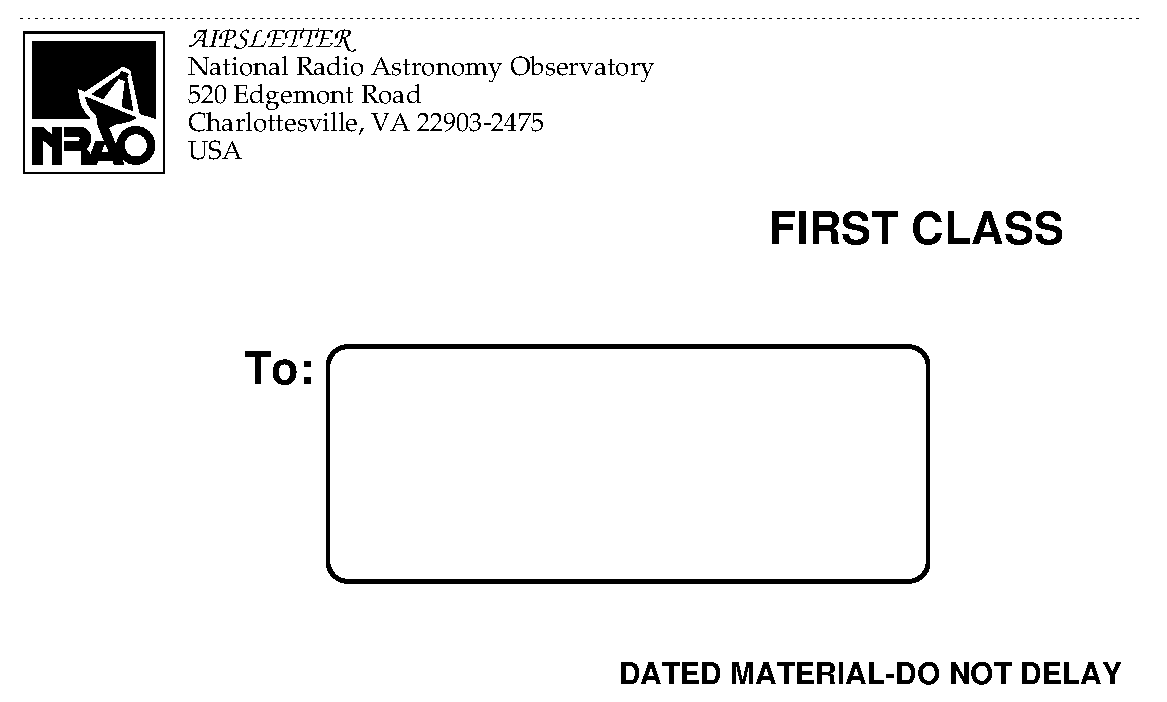
\includegraphics{FIG/AIPSLETM.PS}}}

\end{document}
